\chapter{Desenvolvimento}
\label{cap:desenvolvimento}

\colorlet{punct}{red!60!black}
\definecolor{background}{HTML}{EEEEEE}
\definecolor{delim}{RGB}{20,105,176}
\colorlet{numb}{magenta!60!black}

\lstdefinelanguage{json}{
    basicstyle=\normalfont\ttfamily,
    numbers=left,
    numberstyle=\scriptsize,
    stepnumber=1,
    numbersep=8pt,
    showstringspaces=false,
    breaklines=true,
    frame=lines,
    backgroundcolor=\color{background},
    literate=
     *{0}{{{\color{numb}0}}}{1}
      {1}{{{\color{numb}1}}}{1}
      {2}{{{\color{numb}2}}}{1}
      {3}{{{\color{numb}3}}}{1}
      {4}{{{\color{numb}4}}}{1}
      {5}{{{\color{numb}5}}}{1}
      {6}{{{\color{numb}6}}}{1}
      {7}{{{\color{numb}7}}}{1}
      {8}{{{\color{numb}8}}}{1}
      {9}{{{\color{numb}9}}}{1}
      {:}{{{\color{punct}{:}}}}{1}
      {,}{{{\color{punct}{,}}}}{1}
      {\{}{{{\color{delim}{\{}}}}{1}
      {\}}{{{\color{delim}{\}}}}}{1}
      {[}{{{\color{delim}{[}}}}{1}
      {]}{{{\color{delim}{]}}}}{1},
}

Antes de implementar os métodos analisados, é necessário definir qual cenário será considerado e qual aplicação será alvo dos métodos. Este capítulo tem como base definir este modelo de jogo e especificar quais atributos foram levados em consideração na produção do \textit{software}. Além disso, este capítulo demonstra como o jogo foi modelado, e como os métodos foram construídos a partir do cenário estabelecido. 

A definição formal de um jogo pode ser compreendida como qualquer atividade que exiga um jogador e regras que devem ser seguidas. A definição de um jogo \textit{online}, por sua vez, pode ser interpretada como um jogo que pode ser jogado utilizando uma rede de computador, possibilitando com que dois ou mais jogadores participem simultaneamente de uma partida mesmo estando em lugares diferentes. Este conceito pode ser aplicado para qualquer \textit{software} de jogo, tanto \textit{single-players} (jogos eletrônicos para um jogador) como \textit{online}.

A definição utilizada neste trabalho consiste em uma aplicação que utiliza troca de mensagens entre cliente e servidor, em que o cliente interage com a aplicação por meio de suas ações no jogo. As ações escolhidas são enviadas ao servidor e informadas aos outros jogadores que estão conectados na partida. Para simplificar a construção do \textit{software} e pela irrelevância para os métodos estudados, o ambiente virtual e gráfico do jogo foi desconsiderado em sua implementação.


\section{Jogo}
\label{shoterman}

O jogo projetado e implementado é um jogo de tiro (mais conhecido no cenário de jogos como \textit{shooter}), subgênero de jogos de ação, chamado de \textit{Shooterman}, em que o foco principal do jogo se encontra nas ações que o personagem executa usando algum tipo de arma. No jogo, cada personagem possui uma arma de longa distância, com a qual pode atirar outros jogadores, derrotando-os, e assim, adquirindo pontos de vitória.

Apesar de \textit{Shooterman} não possuir interface visual, é importante salientar que ele é um jogo com perspectiva \textit{top-down}, estilo de jogo em que a câmera encontra-se acima do mapa e o jogador visualiza o cenário de uma perspectiva superior. Esta distinção é importante para a implementação adequada da movimentação dos jogadores e dos projéteis que irão atirar. Afinal, suas coordenadas devem condizer com a perspectiva da câmera do jogo. A mêcanica básica do jogo consiste na interação de vários jogadores no mesmo cenário, podendo se movimentar e atirar entre si, e bloquear tiros que estão chegando ao seu alcance. Tanto o escudo que bloqueia os tiros, como os tiros em si possuem um tempo de recarga, prevenindo que os jogadores utilizem constantemente o escudo ou atirem diversos tiros em um curto espaço de tempo. O último jogador que sobreviver no cenário é o vencedor.


\begin{figure}[h!]
  \begin{center}
    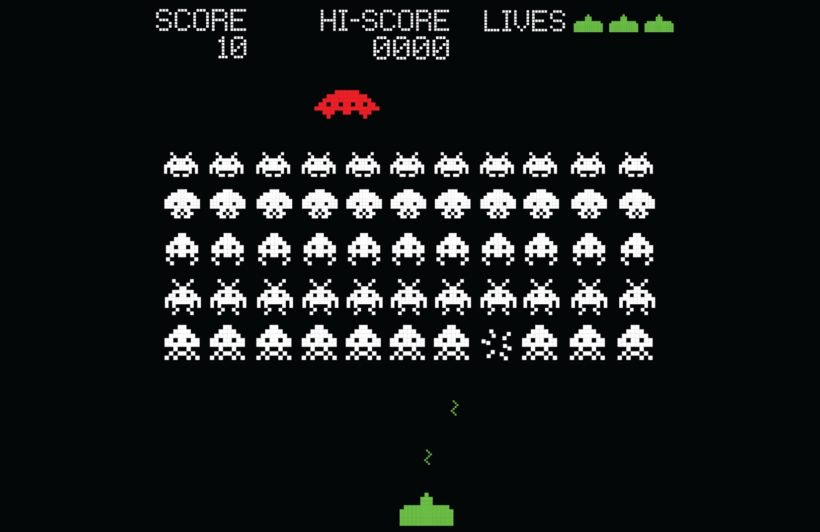
\includegraphics[width=0.6\textwidth]{imagens/space_invaders.jpg}
    \caption{Gameplay do clássico Space Invaders - Exemplo de jogo com câmera top-down.}
    \label{fig:space} 
  \end{center}
\end{figure}


\subsection{Ações do Jogador}

Cada jogador controla um único personagem, que pode atirar projéteis, bloqueá-los e movimentar-se pelo mapa.

O jogador pode movimentar-se em um cenário bidimensional em quatro direções ortogonais - esquerda, direita, baixo e cima. Sempre que ele se movimenta para uma direção, a direção atual que ele está olhando é atualizada. Esta direção será a direção que os projéteis que ele atirar irão seguir.

 A ação principal do personagem é o seu tiro. Quando atira, um projétil é criado a partir de sua posição e atravessa o cenário até colidir com algum objeto ou exceder seu deslocamento máximo. Sempre que o personagem atira, ele não pode atirar novamente por um determinado intervalo de tempo - sua habilidade encontra-se em tempo de recarga.

 O personagem pode também ativar um escudo, uma manobra defensiva, que dura um determinado período de tempo, prevenindo o jogador de ser atingido por ataques inimigos. Este escudo também possui um tempo de recarga que deve ser respeitado.

 Nenhuma dessas ações pode ser executada em um mesmo intervalo de tempo, ou seja, movimentar-se enquanto atira ou atirar enquanto utiliza seu escudo são ações inválidas de acordo com as regras estabelecidas.  



\subsection{Implementação}

Duas aplicações foram implementadas na linguagem C++ versão 11: a versão do cliente e a versão do servidor. Na implementação de \textit{Shooterman}, a autenticidade das mensagens, tanto do cliente quanto do servidor, não foram levadas em consideração da implementação dos métodos. Apesar da transmissão de pacotes utilizar o protocolo UDP, a falha do envio de pacotes também foi descartada para simplificar a implementação dos métodos e avaliar suas funções primárias.


Todas ações executadas pelos jogadores foram enviadas do cliente ao servidor em um \textit{json}. Foi utilizada a biblioteca \textit{JSON for Modern C++}, para facilitar a criação de \textit{jsons} e sua desconstrução em dados brutos utilizados na aplicação \cite{json}. 

\begin{ilustracao}[h!]
  \begin{lstlisting}[language=json,firstnumber=1]
  {
    "player_id" : 4,
    "position": {
      "x" : 5,
      "y" : 8,
      "side" : 0
    },
    "shoot" : "false",
    "barrier_on" : "true"
  }
  \end{lstlisting}
  \caption{Estrutura json utilizada}
  \label{fig:json}

\end{ilustracao}

\lstset {
    language=C++,
    backgroundcolor=\color{black!5},
    basicstyle=\footnotesize,
}

A Figura \ref{fig:json} representa o conteúdo dos dados enviados ao servidor. O mesmo padrão é utilizado pelo servidor ao repassar a mensagem para os outros jogadores, que recebem o arquivo e atualizam as informações do jogo de acordo os dados recebidos. A variável \textit{position} é responsável por representar a posição geográfica do personagem e o lado que ele se encontra. \textit{Shoot} e \textit{barrier\_on} são booleanos de controle que verificam se o jogador está atirando ou ativando sua barreira. \textit{Player\_id} faz referência ao id do jogador que está realizando sua ação. 

No servidor, a classe principal \textit{Game} verifica a cada instante de tempo se um novo cliente conectou-se na aplicação. Sempre que uma nova conexão inicia-se, uma instância da classe \textit{Connection} é criada, onde ela dispara uma \textit{thread} para processar a nova comunicação cliente-servidor, enquanto paralelamente a \textit{thread} principal continua averiguando por novas conexões. A Figura \ref{fig:mainServer} representa a conexão utilizando a classe ServerSocket. Caso o server aceite o novo socket, uma conexão é criada e adicionada a lista de conexões, e uma \textit{thread} é disparada na função newPlayerConnection().

\begin{ilustracao}
    \begin{lstlisting}

        while (true){
            ServerSocket* new_sock = new ServerSocket();
            server->accept (*new_sock);

            try {
                Connection* con = new Connection(this, new_sock, client_id);
                client_connections.push_back(con);
                cout << "Cliente " << client_id  << " conectado!" << endl;
                con->newPlayerConnection();
                client_id++;
            }
            catch (SocketException&) {
                cout << "Erro na conexao com cliente" << endl;
            }
        }
    \end{lstlisting}
    \caption{Thread principal do servidor}
    \label{fig:mainServer}
\end{ilustracao}

Logo quando uma conexão é estabelecida, o servidor envia ao cliente a posição de seu personagem, junto com seu id que será utilizado para identificar seu personagem dentre os outros. Nota-se que o identificador deve ser único para que haja integridade no estado do servidor. Em uma versão mais refinada, em que os clientes cadastram-se na aplicação e possuem seus dados registrados em um banco de dados do servidor, a identificação torna-se mais legítima, afinal, os jogadores teriam seus identificadores únicos registrados junto com informações de suas contas, e utilizariam o mesmo identificador para diversas partidas realizadas na aplicação. Na versão atual, entretanto, os identificadores são provisórios e só se limitam a uma única conexão.

A classe \textit{Connection} é responsável pela comunicação com o cliente conectado, com sua \textit{thread} recebendo mensagens do cliente e retornando suas requisições. Sempre que uma nova mensagem é recebida, ela é validada e enviada a todos jogadores se for considerada semanticamente correta. Percebe-se que dependendo da implementação utilizada no servidor, a função \textit{msgIsValid} varia. Em um cenário que o cliente não possui nenhuma autoridade sobre suas ações, a função avaliaria todas condições necessárias para a ação ser executada, checando sua integridade, e permitindo a ação caso a considerasse legítima. Na versão base da aplicação, entretanto, só é avaliado se o personagem que está realizando a ação realmente é o mesmo controlado pelo usuário da conexão, a partir de seu identificador id. A Figura \ref{mainserver} ilustra a função de comunicação, com a \textit{thread} executando as operações da função update.


\begin{ilustracao}
    \begin{lstlisting}
    void Connection::update(){
      while (true){
        std::string received\_msg;
        *(server_socket) >> received_msg;

        *(player_log) << received_msg << endl;

        auto msg\_json = json::parse(received_msg);
        if (msgIsValid(msg_json) == true){
          updatePlayer(msg_json);
          game->sendToClients(msg_json);
        }
        else{
          cout << "usuario invalido" << endl;
        }
      }
    }
    \end{lstlisting}
    \caption{Função update da classe Conexão responsável pela comunicação cliente servidor}
    \label{mainserver}
\end{ilustracao}


No cliente, a classe principal da aplicação que controla basicamente seu fluxo de operações também é a \textit{Game}. Todos \textit{inputs} do usuário, bem como as comunicações existentes com o servidor operam nesta classe, semelhantemente a classe \textit{Connection} do servidor. Em cada ciclo de execução do cliente, a classe \textit{Game} cuida para que todas suas informações sejam enviadas ao servidor, e que a resposta dele juntamente que contém informações de outros clientes sejam interpretadas e executadas na aplicação.

Sempre que o jogador pressiona uma tecla para atirar, e o cliente pode atirar,  a classe \textit{Game} garante que essa informação seja submetida ao servidor. Essas ações e as verificações que a própria aplicação do cliente faz são executadas na classe \textit{Player}. Esta classe basicamente avalia as ações executadas pelo cliente, e possibilita suas execuções. A classe, por exemplo, verifica se o jogador pode usar seu escudo, ou se ele se encontra indisponível por ter sido utilizado recentemente. Algumas funções e variáveis importantes são ilustradas na Figura \ref{fig:clienteCode1}.

\begin{figure}

  \begin{lstlisting}
  private:
    void toServer();
    void shoot();
    void barrier();
    void checkCooldown();
    void createBullet();

    int side;
    int id;
    bool is_dead = false;
    bool barrier_on = false, can_barrier = true;
    bool can_shot = true, shot = true;

    int shield_cooldown = 0;
    int shot_cooldown = 0;

    const int max_shot_cooldown = 5;
    const int max_shield_cooldown = 15;
    const int shield_time = 5;
    const int player_movespeed = 3;
  \end{lstlisting}

  \caption[Exemplo do arquivo-interface da classe Player da aplicação do cliente.]{Exemplo do arquivo-interface da classe Player.}
  \label{fig:clienteCode1}  

\end{figure}

Todos objetos existentes no jogo, ou mesmo novos objetos que podem ser adicionados futuramente, herdam da classe \textit{GameObject}, que basicamente utiliza a classe \textit{Position}, possibilitando a movimentação dos objetos pelo cenário.

No jogo, somente uma ação pode ser executada por vez, e ações que estiverem em tempo de recarga estarão desabilitadas. Propositalmente, estes testes são verificados no próprio cliente do jogo, então, modificando-o, o cliente pode burlar essas regras, e por exemplo, atirar tiros em um intervalo de tempo menor do que o correto, ou usar seu escudo mais frequentemente que seus adversários.

Todas ações executadas por um cliente são armazenadas em um arquivo, que por sua vez, são analisados com alguns dos métodos estudados no Capítulo 3.


Para facilitar a implementaçãos dos métodos e poder analisar somente seu tempo de processamento, utilizou-se um histórico de mensagens, contendo mensagens enviadas de um cliente ao servidor referente as suas ações executadas. 

\section{Implementação com Execução Simbólica}

\label{implementsimbolic}

Para implementar uma verificador simbólico, deve-se construir uma execução simbólica sobre a aplicação alvo. Visando facilitar os testes e a identificação do custo computacional das verificações das mensagens do cliente, elas foram armazenadas em um arquivo chamado \textit{log}. Neste arquivo, estão armazenadas todas ações executadas por um cliente ao longo de \textit{n} ciclos, onde \textit{n} é o número de linhas do arquivo, e em cada linha dispõe-se a ação realizada. Para gerar o \textit{log}, rodou-se a aplicação do cliente e do servidor durante vários minutos, fazendo com que o cliente faça ações aleatórias em cada um de seus ciclos, enquanto o servidor as armazena no arquivo \textit{log}. Assim, construiu-se uma sequência de ações válidas no arquivo \textit{log}, que foi lida pelo executável simbólico criado. Esta estratégia simula a validação das mensagens do cliente a partir de seu \textit{log} gerado, ou seja, é uma verificação posterior às ações realizadas pelo jogador. Para melhorar o desempenho deste tipo de estratégia, pode-se rodar o algoritmo em apenas parte do \textit{log} armazenado, ou quando se desconfia de um cliente específico após evidências negativas dele vindas de outros clientes. 


O programa usado para gerar a execução simbólica de \textit{Shooterman} foi KLEE, uma máquina virtual simbólica que é construída sobre a estrutura de um compilador LLVM, e disponível gratuitamente\footnote{www.klee.com}. KLEE é baseado em um resolvedor de restrições STP, que implementa uma lógica para encontrar a solução dos conjuntos de restrições impostas a variáveis através da execução simbólica. Para facilitar sua instalação, o KLEE foi utilizado em uma imagem do Docker\footnote{https://www.docker.com/}. Docker é uma plataforma \textit{Open Source} que facilita a criação e administração de ambientes isolados. A partir da imagem obtida do KLEE, foi possível criar um container, contendo o necessário para a utilização das ferramentas e bibliotecas disponíveis da máquina virtual simbólica.  


Para o programa ser executado na máquina simbólica, ele deve primeiramente ser compilado como um arquivo \textit{bitcode} no formato LLVM. Para isso utilizou-se o Clang++, com a \textit{flag} -emit-llvm.  Como vários arquivos são utilizados, usou-se o \textit{llvm-link} para permitir que vários arquivos \textit{bitcode} LLVM juntem-se em um único arquivo \textit{bitcode} \footnote{https://llvm.org/docs/index.html}. Infelizmente, apesar do KLEE reconhecer o arquivo \textit{bitcode} gerado como válido, ele não reconheceu chamadas externas de funções e construtores de outras classes, retornando uma falha de chamada externa logo na construção da primeira classe instanciada.

Para prosseguir com a implementação, o código criado foi modificado para ser compatível em C. Para facilitar essa modificação, somente os arquivos mais essenciais do controle do fluxo do jogo foram convertidos, ocupando o único arquivo 
\textit{client\_main.cpp}. Como a biblioteca \textit{JSON for Modern C++} não pôde ser utilizada, rodou-se um \textit{script} em Python para converter os dados no formato \textit{json} em um formato mais prático de ser lido em C. O A partir deste novo arquivo, pode-se ler linha por linha do arquivo, atribuindo os valores lidos para variáveis usando a função \textit{sscanf} do C. 

Na implementação, somente a variável \textit{action} é representada simbolicamente. Nota-se que na Figura \ref{fig:clienteCodeSimbolica}, a variável \textit{action} representa uma ação que o jogador tomou. Como torna-se simbólica, ela pode representar qualquer valor, variando de 0 a 5, refletindo consequentemente uma das ações possíveis realizadas pelo jogador. A função \textit{randomMovement()} desta implementação atualiza as informações do personagem de acordo com a ação realizada. Basicamente, ela executa a ação passada como parâmetro (a variável simbólica \textit{action}) e determina se o resultado da ação é equivalente com os resultados armazenados na variável \textit{line}. Como a ação é simbólica, considera-se que todas ações possíveis do jogador foram testadas, e se uma delas resultou na equivalência com a ação registrada no log, a ação registrada no log é considerada semanticamente autêntica.

 O retorno dessa função \textit{randomMovement()} retorna a validação da ação. Como cada valor possível de \textit{action} cria um novo ramo de execução, o ramo deve ser finalizado se mostrar-se inválido semanticamente, por isso a função é retornada caso aquela ação seja considerada inválida. Os valores válidos, entretanto, continuam executando e ramificando novamente, na próxima iteração do \textit{while}.

\begin{figure}[h!]
    \begin{lstlisting}
        while ((read = getline(&line, &len, file)) != -1){
            klee_make_symbolic(&action, sizeof(action), "action");
            if (randomMovement(action, line) == false)
                return;
        }
    \end{lstlisting}
    \caption{Exemplo do código de execução simbólica usando KLEE.}
    \label{fig:clienteCodeSimbolica}  

\end{figure}

Em cada iteração do código da Figura \ref{fig:clienteCodeSimbolica}, o próprio KLEE gera restrições sobre a ação \textit{action} executada, determinando se ela deve ser ignorada ou não. Como todas ações possíveis são verificadas, o número de restrições aumenta conforme o número de possibilidades que o jogador poderia executar em cada um de seus ciclos. Na abordagem utilizada, o número de restrições continua a aumentar conforme o número de ações é verificado, fazendo com que o número de ramos de execução gerados seja muito grande, contendo informações duplicadas de possíveis ramos que acabarma falhando em identificar a próxima ação executada. 


\section{Implementação do SSIP}
\label{implementsemantic}

A partir da definição de estados abstratos e concretos do Capítulo \ref{cap:definicaoestado}, pode-se comparar as informações enviadas ao servidor de \textit{Shooterman} como abstratas e as informações contidas no cliente como concretas. Levando em consideração, por exemplo, o escudo que o jogador pode ativar para tornar-se imune aos projéteis inimigos, o servidor somente tem acesso a informação da ativação do escudo, e não de seu tempo de recarga. Em jogos mais complexos, outras informações associadas às ações do jogador, como colisões que podem ocorrer durante uma movimentação do personagem, também podem ser consideradas como informações concretas. Mas, se estas ações fossem enviadas diretamente ao servidor e verificadas lá em cada um dos ciclos do cliente, ocasionariam um processamento extensivo demais para ser realizado pelo servidor. 

Como a autenticidade dos usuários não foi levada em consideração, o uso de \textit{hashs} e autenticadores de mensagens foi desconsiderado tanto na implementação quanto nos custos atribuídos a utilização deste método. 

Analisando o SSIP, percebe-se que para realizar a verificação dos estados do cliente, o servidor de auditoria deve possuir acesso ao estado concreto inicial do cliente (referente ao Protocolo de Inicialização, Capítulo \ref{protocoloinicializacao}), acesso a todas \textit{diffs} entre os estados concretos de $t_a$ a $t_0$, assim como acesso a todas \textit{diffs} entre os estados abstratos de $t_a$ a $t_0$.

Modificando o cliente, foi criado um arquivo durante sua conexão com o servidor, que armazena informações dos estados concretos, \textit{diffs} abstratas e \textit{diffs} concretas de todos estados ao longo de uma partida. 
Este histórico de estados é então lido por um programa, que na prática atua como um servidor de auditoria. Após ler os conteúdos correspondentes aos estados e $\Delta$'s, os passos do protocolo de auditoria (mais detalhes no Capítulo \ref{protocoloAuditoria}) foram executados para verificar a integridade dos estados. 

Primeiramente, a partir do estado concreto inicial, são calculados todos estados concretos a partir das \textit{diffs} concretas obtidas. 
Como todos estados foram armazenados no formato \textit{json}, foi relativamente fácil de atribuir as mudanças $\Delta$ aos estados. A figura \ref{clientestep} ilustra o processo do quarto passo do protocolo de auditoria do Capítulo \ref{protocoloAuditoria}. A figura \ref{fig:exa} ilustra a forma abstrata e concreta de definir informações do jogo. Na primeira linha, é informado a nova posição do jogador após sua movimentação. Informações adicionais, como o tempo de recarga atual de outras habilidades só é retratado nas mensagens concretas, como a segunda linha demonstra. 


\begin{figure}
    \begin{lstlisting}
        auto a = concrete_states.begin();

        next_states.push_back((*a));

        auto delta = concrete_delta.begin();
        string actions[] = {"position", "barrier", "can_barrier", "shield_cooldown", 
        "shoot", "can_shot", "shot_cooldown"};

        for (delta; delta != concrete_delta.end(); delta++){
            json new_state;

            json delta_json = (*delta);

            for (string s : actions){
                if (delta_json.count(s) != 0){
                    new_state[s] = delta_json[s];
                }
            }

            next_states.push_back(new_state);
        }

    \end{lstlisting}
    \caption[Exemplo de criação dos estados a partir do estato concreto e $\Delta$ concretos.]{Exemplo de criação dos estados a partir do estato concreto e $\Delta$ concretos.}
    \label{clientestep}  
\end{figure}


\begin{figure}
  \begin{lstlisting}[language=json,firstnumber=1]
    {"position":{"side":0,"x":-8,"y":8}}
    {"position":{"side":0,"x":-8,"y":8},"shield_cooldown":1}
  \end{lstlisting}
  \caption{Exemplo de diffs abstratas e concretas}
  \label{fig:exa}
\end{figure}


A parte que demanda maior custo computacional deste protocolo é o quinto passo, onde é verificado se cada $\Delta$ concreto é válido ou não. Neste modelo, a partir de cada estado do jogo, é verificado se as ações executadas condizem com a integridade e as regras que a NVE deve cumprir. Ou seja, para cada mudança concreta ocorrida, é analisado se ela poderia ter ocorrido ou não, ou se outra mudança deveria ocorrer no lugar. Um exemplo simples disso seria da utilização da barreira. Caso ela tenha sido usada em um ciclo anterior, os próximos \textit{diffs} concretos devem manter a atualização do tempo de recarga da barreira, até ela poder voltar a ser utilizada. Se o tempo de recarga não apareceu entre uma \textit{diff} e outra após o cliente ter usado sua barreira, ou se a diferença do tempo de recarga entre uma \textit{diff} e outra é maior do que um, conclui-se que o jogador está escondendo informações ou modificando os dados no cliente de jogo.